%---------------------------------------------------------------------------%
%->> Frontmatter
%---------------------------------------------------------------------------%
%-
%-> 生成封面
%-

\maketitle% 生成中文封面
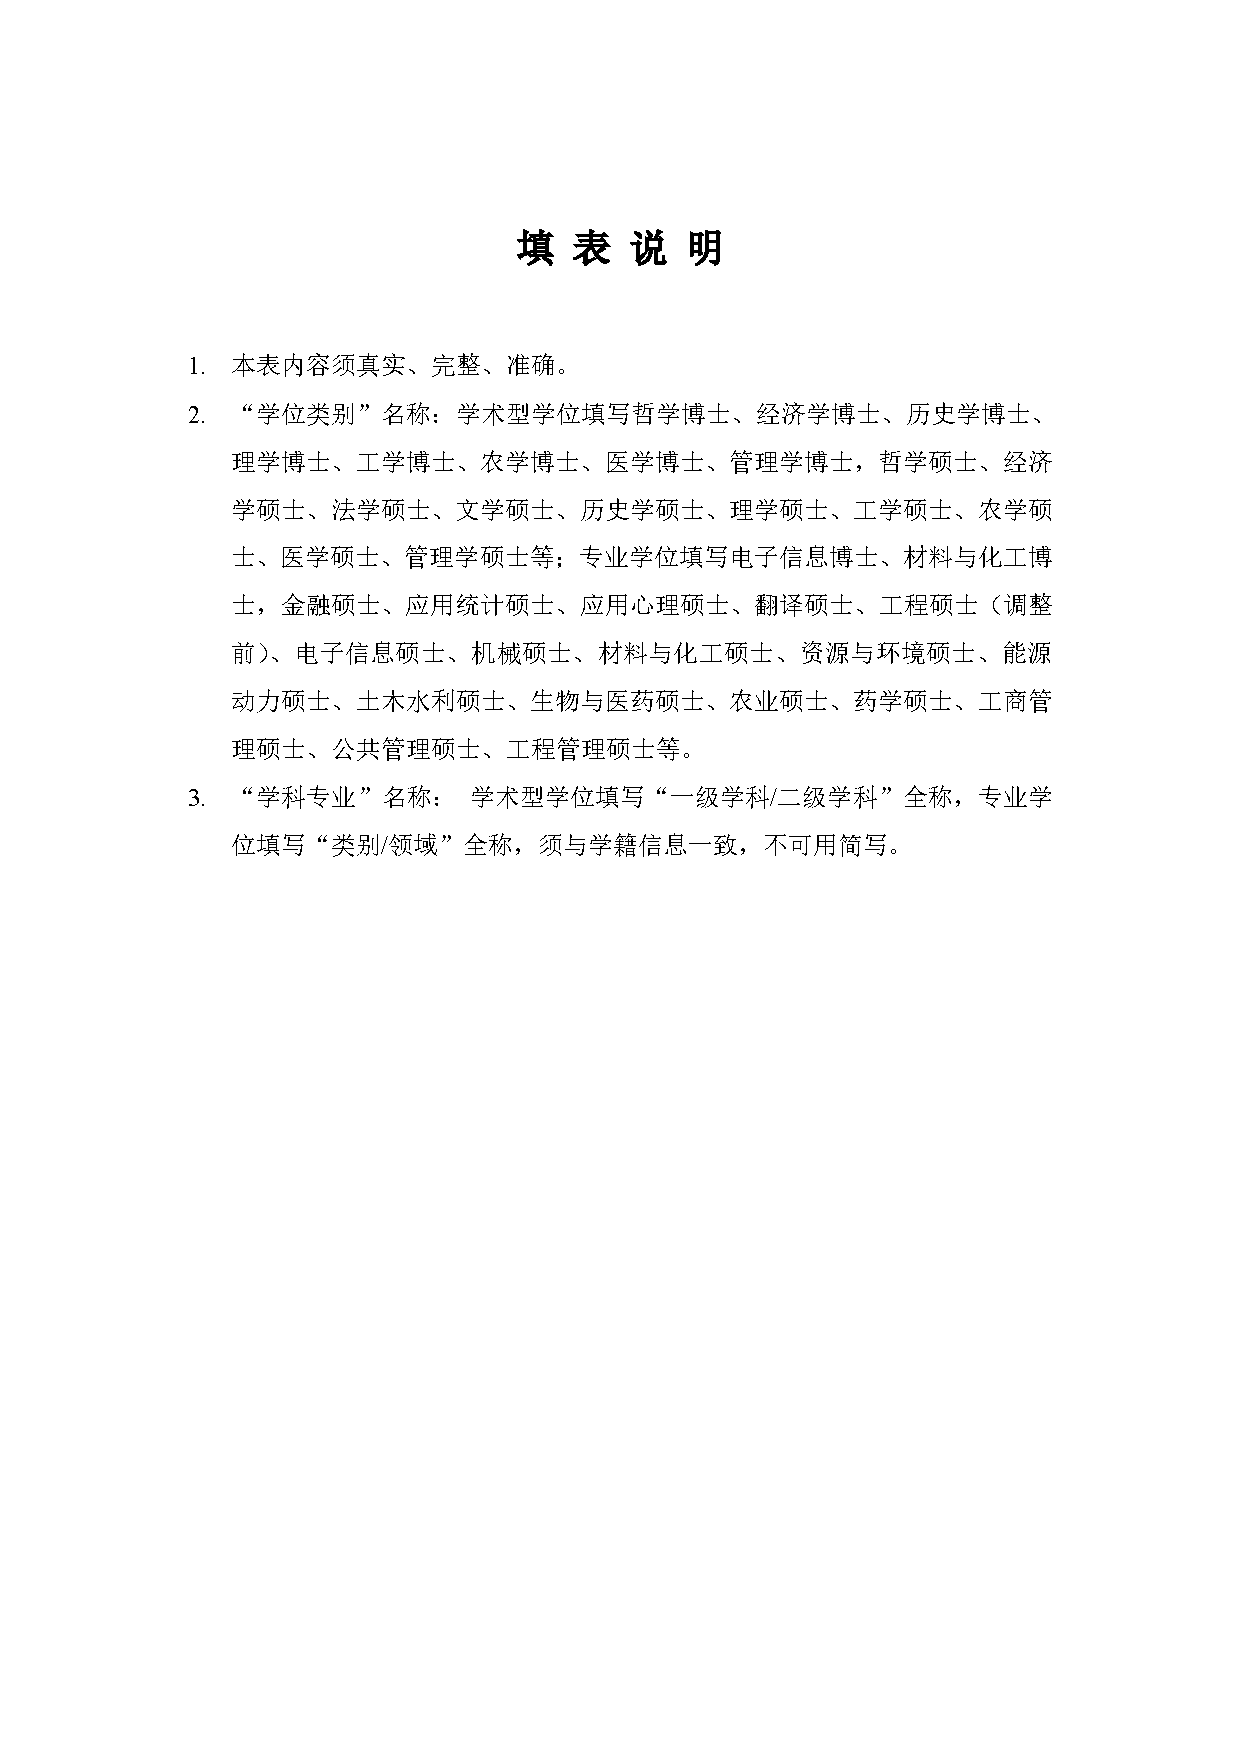
\includepdf[pages=1-2]{Tex/Interim.pdf}
% \MAKETITLE% 生成英文封面
% %-
% %-> 作者声明
% %-
% \makedeclaration% 生成声明页
% %-
% %-> 中文摘要
% %-
% \intobmk\chapter*{摘\quad 要}% 显示在书签但不显示在目录
\setcounter{page}{1}% 开始页码
\pagenumbering{Roman}% 页码符号

% 中文摘要、英文摘要、目录、论文正文、参考文献、附录、致谢、攻读学位期间发表的学术论文与其他相关学术成果等均须由另页右页(奇数页)开始。

% \keywords{中国科学院大学,学位论文,模板}% 中文关键词
% %-
% %-> 英文摘要
% %-
% \pagestyle{frontmatterstyle}%
% \intobmk\chapter*{Abstract}% 显示在书签但不显示在目录
% \pagestyle{enfrontmatterstyle}%

% Chinese abstracts, English abstracts, table of contents, the main contents, references, appendix, acknowledgments, author's resume and academic papers published during the degree study and other relevant academic achievements must start with another right page (odd-numbered page).

%     %- the current style, comment all the lines in plain style definition.

% \KEYWORDS{University of Chinese Academy of Sciences, Thesis, LaTeX Template}% 英文关键词

% \cleardoublepage\pagestyle{frontmatterstyle}%
% \cleardoublepage
\clearpage

%---------------------------------------------------------------------------%
